

\documentclass[12pt]{article}
\usepackage[T1]{fontenc}
\usepackage[utf8]{inputenc}
\usepackage{amsmath}
\usepackage{microtype}
\usepackage{listings}
\setlength{\parindent}{0pt}
\usepackage{fancyvrb}
\usepackage{enumerate}
\usepackage{array}
\usepackage[breaklinks=true,linktocpage,hidelinks]{hyperref}
\usepackage[letterpaper]{geometry}
\usepackage{url}
\usepackage{graphicx}
\usepackage{fullpage}

\usepackage{pgfplots}
\usepackage{pgfplotstable}
\usepackage{tikz}

\usepackage{fancyhdr}
\usepackage{fancybox}
\usepackage{multicol}
\usepackage{xcolor}
\usepackage{adjustbox}

\pgfplotsset{compat=newest}
\usetikzlibrary{shapes,backgrounds,arrows}
\usepgfplotslibrary{external} 

\definecolor{brewcol1}{RGB}{166,206,227}
\definecolor{brewcol2}{RGB}{31,120,180}
\definecolor{brewcol3}{RGB}{178,223,138}
\definecolor{brewcol4}{RGB}{51,160,44}
\definecolor{brewcol5}{RGB}{251,154,153}
\definecolor{brewcol6}{RGB}{227,26,28}
\definecolor{brewcol7}{RGB}{237,179,1}
\definecolor{brewcol8}{RGB}{202,178,214}
\definecolor{brewcol9}{RGB}{206,27,1}

\geometry{hmargin=1.87cm, vmargin=1.87cm}
\bibliographystyle{siam}

\DeclareTextFontCommand{\helvetica}{\fontfamily{phv}\selectfont\small}


\begin{document}

\clearpage\thispagestyle{empty}
\begin{center}
\textbf{Difficult transition for sugar maple in Boreal forest under climate change? \\
Impact of alternative stable states on Sugar maple migration.}
\vskip 2em
Research proposal
\vskip 1em
Master in Wildlife management
\vfill
By
\vfill
Steve Vissault 
\vfill 
For
\vfill
\textbf{Richard Cloutier}, Pr.\\
Director of the program committee
\vskip 2em
\textbf{Dominique Arsenault}, Pr.\\
President of the jury
\vskip 2em
\textbf{Matt Talluto}, PhD\\
Research Co-director
\vskip 2em
\textbf{Dominique Gravel}, Pr.\\
Research Director
\vfill
\vfill
Université du Québec à Rimouski\\
\today

\end{center}

\newpage
\setcounter{page}{1}

\section{Introduction}

\textbf{Context.} Sugar maple (\textit{Acer saccharum}) is a widespread and
abundant tree species in north-eastern North America.
\cite{Graignic2013,Messaoud2007,Kellman2004,Barras1998}. Predicting shifts in
the range of Sugar maple is of prime importance because this species is highly
desirable for hardwood and maple syrup production, two large economic sectors
in Quebec. This species is dominating the temperate forest up to the boreal-
temperate ecotone at its northern range limit \cite{Barras1998}. Some
representative species of northern forest ecosystems are expected to expand
their distribution towards the north following climate warming
\cite{Sciences2014,Iverson2002}. According to McKenney (2007)
\cite{Sciences2014}, the climatic conditions  favorable to Sugar maple  will
reach the Ungava bay within the next 100 years, which appears highly
improbable because of dispersal limitations and slow population dynamics.
Such predictions are built on species distribution models accounting only for
climatic conditions; it is recognized that Sugar maple regeneration depends
both on macro  (\textit{i.e.} regional climate) and micro environmental
conditions (\textit{i.e.} soil and microtopography)
\cite{Graignic2013,Lafleur2010}. Thus, the expansion of Sugar maple and iis
difficult to predict because micro conditions can mitigate macro conditions
such as global warming \cite{DeFrenne2013}.\\ 
%DG: la dernière phrase n'est pas claire, je n'ai pas réussi à l'éditer comme la précédente.

Soil-plant feedbacks are susceptible to impact Sugar maple migration dynamics.
Tree species respond differently to the soil conditions, and the soil
properties found in boreal forests are different from those in temperate
forest \cite{Lafleur2010,Barras1998,Goldblum2010,Demers1998}. A deep and
poorly-decomposed litter layer is usually found in boreal forests, while the
litter of  northern hardwood forests is thinner and mainly composerd of a
superficial leaf mat \cite{Barras1998}. The temperature is colder, the snow
melts later and the soil is wetter under coniforous trees
\cite{Lafleur2010,Goldblum2010}. Soil acidification causes a reduction in the
cation exchange capacity and subsequently decreases availability of some
nutrients such as calcium \cite{Moore2008}. Sugar maple seedlings have been
recognized to be particularly sensitive to waterlogged conditions and soil
nutrient content \cite{Moore2008,Lafleur2010,Cleavitt2011}. These properties
of coniferous forest soils could hinder the local establishment of species
associated with alkaline soils or unable to withstand waterlogged conditions
\cite{Lafleur2010}. Under these conditions, tree species migration is likely
to be restricted or delayed \cite{Lafleur2010}. Thus, even if the climatic
conditions at the regional scale become favorable to Sugar maple after climate
warming, the micro conditions found in the boreal forest could slow seedling
establishment \cite{Kellman2004,Moore2008,Barras1998,Messier2011}.Sugar maple
could thus be unable to colonize the boreal forests as a result of strong and
localized plant-soil feedbacks \cite{McCarthyNeumann2012}.\\

I hypothesize that the temperate-boreal forest ecotone is as a system
dominated by two alternative states, \textit{i.e.} contrasted states occurring
in the same climate conditions \cite{scheffer2009critical}: the boreal
community and the temperate community, including Sugar maple. The landscape is
made of a patch mosaic where micro conditions are driving the spatial
occurrence of boreal and temperate communities, despite a regional climate
favourable to temperate species \cite{Goldblum2010,Fisichelli2013}. I expect
that a climate warming and the subsequent incapacity of Sugar maple to
colonize boreal forest stands will create  tension between the potential and
realized forest composition and consequently that abrupt shifts in community
composition are susceptible to occur at the boreal-temperate forest ecotone.\\


\textbf{Objectives.} The main objective of this project is to investigate the
transition between the boreal and temperate forests under different climate
change scenarios. In this context, we will test two different hypotheses:
($H_1$) Alternative stable states do co-occur at the boreal-temperate forests
ecotone, and ($H_2$) the response of Sugar maple to climate change will be
delayed in  in areas where alternative stable states are susceptible to occur.
In order to fulfill this objective and test these hypotheses, we will (1)
develop a climate-dependent  state-transition model (STM) representing the
dynamics of the boreal and temperate communities at landscape scale; (2) study
the occurrence of alternative stable states at the temperate-boreal ecotone;
and finally (3) run simulations of the temperate community species
distribution under different climate change scenarios. The first section of
this proposal reviews the context of the study. The first part of the review
presents the concept of alternative stable states and critical transitions in
forest ecosystem properties. The second part focuses on Sugar maple, its
associated community in the temperate biome, and a justification about why
alternative stable states are expected to occur at the boreal-temperate
forests ecotone. The last section of this proposal describes the model and the
methodology that we will employ to achieve the specific objectives.


\section{Review} 

\begin{figure}[t]
	\begin{center}
	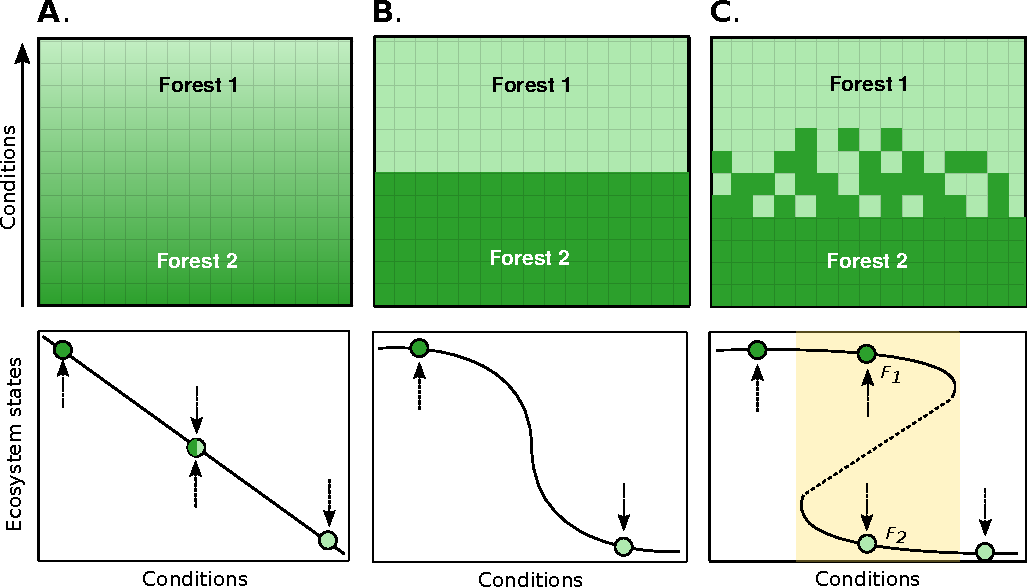
\includegraphics[width=0.8\textwidth]{fig/states.pdf}
	\end{center}
	\caption{Schematic representation of different ways in which the forest-forest ecotone can vary over environmental gradients such as temperature, precipitation
	or soil moisture. Three different responses to an environmental gradient are presented,
	\textbf{(A)} gradual, \textbf{(B)} basic fold, \textbf{(C}) catastrophic fold.
	Upper panels represent the change in the ecosystem state over an environmental gradient. Solid lines represent stable states along the boreal-temperate
	transition, and the dashed line (in yellow highlight) unstable equilibrium. Arrows indicate the
	direction the system moves if not at the equilibrium. The zone with alternate stable states,
	called hysteresis, is unstable and small fluctuations in
	environment conditions give rise to abrupt changes in ecosystem state ($F_1$ or $F_2$). 
	The bottom panels illustrate a conceptualization of a transitional landscape
	between the boreal (light green) and the nordic temperate forests (dark
	green).}
	\label{fig1}
	\vspace{-1.25em}
\end{figure}


\textbf{Alternative stable states in forest ecosystems.} The idea that
alternative stable states may exist in community ecology was proposed in the
late 1960s \cite{Scheffer2001,Society2014a}. May (1977) \cite{May1977}
highlighted the fact than an ecosystem can be seen as a dynamic system where
communities are not constant accross the time and possess several different
equilibrium points or stable states given a specific environnement.


% DG: cette phrase n'est pas claire. Qu'est-ce que tu veux dire par un système
% dynamique? Ensuite, pourquoi tu réfères deux fois à May dans la même phrase?

%DG: attention à la rédaction redondante. La phrase précédente ne fait que
%répéter ce qui est au dessus.

%DG: attention aussi lors de la rédaction, tu as tendance à avoir des
%artifices de langages qui sont inutiles. Simplifie ton texte au max. Par
%exemple, dans la phrase précédente, à quoi sert le 'usefully', 'dynamic', 'a
%set of'? Tu peux retirer ces mots sans changer le sens de la phrase, en fait
%même ça va l'alléger. J'ai fait plusieurs petites corrections ici et là, tu
%devras apprendre à simplifier ton texte. Ici ce n'est plus une question de
%traduction anglais/français, c'est vraiment d'écrire le plus efficacement
%possible, sans artifices.

%DG: idem pour la phrase précédente, 'species' est inutile. Par ailleurs,
%cette définition n'est pas vraiment claire. Réviser.

There are three possible responses of ecosystems to changing environmental
conditions: \textbf{(A)} gradual, \textbf{(B)} basic fold, \textbf{(C})
catastrophic fold  \cite{Scheffer2001} (Figure \ref{fig1}, upper line).

%DG: cette phrase par exemple serait plus claire si retournée: There are three
%possible responses of ecosystems to changing environmental conditions

First, when a small modification environmental occurs, the state of the forest ecosystem can
change almost linearly (Figure \ref{fig1}.a, upper line)
\cite{Scheffer2001,Scheffer2009}. In this case, ecosystems can be seen
as a continuum of states along the climate gradient
\cite{Scheffer2001,Scheffer2009,scheffer2009critical}.

%DG: c'est quoi cette histoire de précipitations et de transition décidue/tempéré?

Secondly, the ecosystem can be insensitive to
changing environmental conditions over a certain range, but respond
strongly when a threshold is reached \cite{scheffer2009critical}. 

% DG: c'est répétitif tout ça, tu peux couper pas mal de texte. Mais tu
% devrais aussi en rajouter en expliquer les facteurs responsables de ces
% différentes réponses.

Lastly, in some non-linear systems, the response curve can be folded backwards
and alternative stable states could occur (Figure \ref{fig1} .c). When the
system approaches a tipping point on the folded upper branch, it cannot pass
smoothly to the lower branch. Small forcing on initial conditions of the state
$F_1$ transfer the system immediately into a different state $F_2$ (Figure
\ref{fig1} .c). Hence, at this point, the system is particularly sensitive to
the initial conditions. This point is called a bifurcation point and a small
forcing on it can drive the system into backward or forward shifts towards
either alternative stable states \cite{scheffer2009critical}. The main
ingredient to creating alternative stable states is the occurrence of positive
feedbacks \cite{scheffer2009critical,Schroder2005}. One well known is
facilitation in ecological succession (i.e. the idea that pioneer species pave
the way for later successional species) and this feedback seems to be present
in the the boreal-temperate forests studied \cite{Barras1998,Society2014}. \\

% DG: comme Matt le faisait remarqué, ce paragraphe est bizarre parce que tu
% oscilles entre la théorie, des exemples forestiers, et ensuite de vrais
% exemples. Essayer de garder la même logique tout du long. Comme il s'agit de
% la review, je sortirais la forêt du paragraphe et prendrais seulement de
% vrais exemples documentés et faciles à expliquer. Je ferais un paragraphe
% supplémentaire ensuite où je ferais une interprétation en termes forestiers,
% bref, une description des panneaux du bas de ta figure. Ça devrait venir
% j'imagine à la fin de la section Natural system studied. un paragraphe qui
% commence par 'The transition from temperate to boreal forests along a
% climatic gradient could adopt any of the three response curves.'

\textbf{Natural system studied.} Many empirical and modelling studies have been
conducted on the transition between forest to non-forests communities (e.g. Boreal-Tundra) 
\cite{Scheffer2012,Scheffer2001,Hirota2011,Messaoud2007}. Little
attention has been given to understand forest-forest ecotones
\cite{Goldblum2010,Graignic2013,Messaoud2007}. 

%DG: attention aussi aux accords, pluriel etc.... Par exemple, dans la phrase
%suivante, il n'y a qu'une échelle, scale ne devrait pas avoir de s DG: la
%phrase suivante est aussi maladroitement écrite. C'est évident que la forêt
%est un système dynamique, c'est trivial. Tu veux trop en mettre dans cette
%phrase. Tout ce que tu veux dire finalement c'est que chaque type de
%peuplement forestier pourrait être vu comme un état, dont la proporition à
%l'échelle du paysage est susceptible de varier avec les conditions
%environnementales.

At landscape scale, transitions
between  the temperate and boreal forests can be approached as a dynamical
system where each forest biome community is a stable state (Figure \ref{fig1},
lower line). There is no distinct boundary at the boreal-temperate ecotone;
instead a broad transition zone exists where stands of coniferous and
deciduous species co-occur at the regional scale
\cite{Goldblum2010,Fisichelli2013}. 

% DG: ce n'est pas toujours clair ce qui est une hypothèse et ce qui est
% documenté.

A macromosaic landscape can be observed
with either pure stands of northern temperate trees or boreal forest stands
\cite{Goldblum2010,Fisichelli2013}. 

%DG: la phrase suivante est à retravailler, trop d'informations. Tiens-toi à
%sujet verbe complément. Ici tu parles de deux trucs en même temps; d'abord
%qu'on peut appliquer la théorie à ce système et ensuite que les stades
%stables alternatives peuvent être causés par différents facteurs. Sépare ces
%infos dans deux phrases pour éviter de faire une phrase alambiquée

The theory on alternative stable
states could be applied to the hardwood-boreal forest patchiness structure
often attributed to differences in soils, nutrient status and topographical
factors \cite{Society2014}. 

%DG: pourquoi segregated? encore une fois, tu mélanges plusieurs idées dans la
%même phrase.

This segregated patch distribution could be
explained by the fact than microclimatic conditions can modulate establishment
of those forests \cite{DeFrenne2013}. Distribution of deciduous and boreal
forests at the ecotone is not determined by macroclimatic conditions, but
rather by local variation of substrate, drainage, physical soil properties,
and nutrient availability \cite{Goldblum2010,Society2014}. 

%DG: ah bon, la phrase précédente était claire. structure simple, efficace,
%une seule idée.

Boreal and hardwood
forests are dominated by trees with different physiognomy, which is expected
to produce distinctive litter and light micro-environments \cite{Barras1998}.

%DG: physiognomy??? Les arbres ont différentes allures? La définition: The art
%of judging human character from facial features DG: tu mélanges beaucoup les
%hypothèses et les faits dans ce paragraphe. Il faudrait s'assurer de tout
%séparer pour que ce soit plus clair. Je pense que tu devrais séparer cette
%section en deux paragraphes. Tu commences par dire que tu t'attends à des
%stades stables alternatifs en raison de l'écologie des espèces tempérées et
%boréales. Là tu listes tous les faits. Ensuite au paragraphe suivant, tu
%décris tes attentes quant à la transition (panneau du bas de la figure).

A positive feedback contributes to the maintenance of the community type if
the dominant tree species promotes conditions facilitating its own
regeneration \cite{Barras1998}. Frelich \textit{et al.}(1993)
\cite{Society2014} hypothesized such a soil-plant feedback impacts Sugar maple
and hemlock spatial distribution. Hence, soil conditions and role of dominant
species in regeneration seems to act as main feedbacks on the temperate forest
establishment (Figure \ref{fig1}.c, upper panel). Boreal soil can delay
temperate species regeneration (negative feedback) and, on other hand,
temperate species establishment can enrich the soil so they promote their own
regeneration (positive feedback).

%DG: attention, l'effet des espèces boréales est aussi un feedback positif:
%plus il y a de sapin, plus la régénération de sapin est favorisée

In this context, we expect to find forest stands dominated by either boreal
species or temperate species and sensitivity to initial conditions. Thus, the
soil condition and the role of dominant species in boreal and temperate
forests need to be investigate as main drivers in shifts between alternative
stable states \cite{Kellman2004,Moore2008,DeFrenne2013,Barras1998}.

%DG: il manque des explications sur l'impact possible des ASS sur les taux de
%migration.

\section{Methods}   

\begin{wrapfigure}{L}{0.45\textwidth}
	
\begin{center}
	
				\tikzstyle{noeud}=[circle,
				                  thick,
				                  minimum size = 1.5cm,
				                  inner sep =5pt,
				                  draw=brewforest3,
				                  fill=brewforest1]
				\tikzstyle{noeud2}=[circle,
				                  thick,
				                  minimum size = 1.5cm,
				                  inner sep =5pt,
				                  draw=brewforest3,
				                  fill=brewforest3]
				\tikzstyle{noeud3}=[circle,
				                  thick,
				                  minimum size = 1.5cm,
				                  inner sep =5pt,
				                  draw=brewforest3,
				                  fill=brewforest3]
	
				\begin{tikzpicture}[->,>=stealth',auto,scale=0.65]
				      \node [circle,noeud2] (M) at (0,0) {\color{white}\textbf{M}};
				      \node [circle,noeud2]  (C) at (-5,5) {\color{white}\textbf{C}};
				      \node [circle,noeud2] (D) at (5,5) {\color{white}\textbf{D}};
				      \node [circle,noeud2] (T) at (0,10) {\color{white}\textbf{T}};
	
						\draw[thick,-latex] (M) to[bend right=10] node[above,sloped] {$S_C$} (C);
						\draw[thick,-latex] (C) to[bend right=10] node[below,sloped] {$\beta_d \cdot (D+M)$} (M);
	
						\draw[thick,-latex] (D) to[bend right=10] node[above,sloped] {$\beta_c \cdot (C+M)$} (M);
						\draw[thick,-latex] (M) to[bend right=10] node[below,sloped] {$S_D$} (D);
	
						\draw[thick,-latex] (D) to[bend right=10] node[above,sloped] {$e$} (T);
						\draw[thick,-latex] (T) to[bend right=10] node[below,sloped] {$\phi_D$} (D);
	
						\draw[thick,-latex] (T) to[bend right=10] node[above,sloped] {$\phi_C$} (C);
						\draw[thick,-latex] (C) to[bend right=10] node[below,sloped] {$e$} (T);
	
						\draw[thick,-latex,transform canvas={xshift=0.8ex}] (T) to node[above,sloped,rotate=90,transform canvas={xshift=3ex}] {$\phi_M $} (M);
						\draw[thick,-latex,transform canvas={xshift=-0.8ex}] (M) to node[above,sloped,rotate=-90,transform canvas={xshift=-3ex}] {$e$} (T);
				\end{tikzpicture}
	\end{center}	


	\caption{Conceptual representation of the transition model between deciduous ($D$),
	mixed ($M$) and coniferous ($C$) stands. $T$ corresponds to a post-disturbance forest patch. Perturbations, natural and anthropogenic, occur with a frequence $\epsilon$. 
	Flows or transition rates between states are represented by arrows.
	Parameters $\theta$ and $\beta$ are rates of colonization and succession,
	respectively. We define recovery functions $\phi_c$ , $\phi_d$ as $\phi_c
	= \alpha_c \cdot (M+C) \cdot [1- \alpha_d \cdot (D+M)]$ and $\phi_d =
	\alpha_d \cdot (D+M) \cdot [1- \alpha_c \cdot (C+M)]$. $\phi_m$ include these both equations giving $\phi_m = \phi_c \cdot \phi_d$. Finally, parameter $\alpha$ represents the climate-dependent recovery rate after a patch has been disturbed.}
	\label{Model}
	\vspace{-1em}
\end{wrapfigure}


%% NOTE FROM MATT: The following paragraph is still suffering from some organizational difficulties
% It jumps around a bit from one subject to the other, making it very hard for the reader
% to follow the logic. It is important to clearly identify how one sentence leads to the
% next. It is also very important to clearly distinguish the text and the figure--they
% should be independent. Do not describe the figure in the text (that is for the caption),
% and do not describe the model in the caption (unless it is necessary to understand the 
% figure)
%
% STEVE: DOM let me know if that's still unclear, I modified it !


\textbf{State and Transitional Model.} The framework of this study lies is a
STM representing dynamics in the boreal-temperate forest transition at the
landscape scale.  Overall, the ecotone landscape includes three distinctive
kind of forest canopies: (i) deciduous, (ii) mixed and finally (iii)
coniferous \cite{Fisichelli2013}.  Each of these stand types is represented as
a state in the STM: \textbf{(D)} Deciduous, \textbf{(M)} Mixed, \textbf{(C)}
Coniferous and finally we added \textbf{(T)} a Transitional patch detailled
later in the paragraph (green circles, figure \ref{Model}).  According to
Briske\textit{ et al.} (2008) and this STM context, state means a plant
community phase occurring on similar soils that interact with the environment
to produce persistent functional and structural attributes \cite{Briske2008}.
Each transition rates between states are  are climate-dependant. Transitions
between all states are possible except the direct transition between a
deciduous and coniferous stand, which requires an intermediate step through
state M. Except for the colonization rate ($\theta$), transition rates vary
with the proportion of coniferous or deciduous available in the closest
neighbourhood. For instance, the succession rate of a coniferous patch
($\beta_c$) towards a mixed patch (M) depends also on the availability of D
and M patches in the landscape (figure \ref{Model}).  Natural processes such
succession and colonization are not the only mecanisms leading the transition
between two states. In fact, natural disturbances are an important driver of
forest dynamics at landscape scale (e.g. fire in boreal forest or large
windthrow in temperate forest). For instance, small fires induce deciduous
dominance and larger and intense fires favouring boreal communities
\cite{Bergeron2004}. Anthropogenic disturbances such as logging can also
produce major change in the forest composition. Dupuis \textit{et al.} (2011)
revealed that historical disturbances affected the propensity of taxa to
expand (maples/aspen) or decline (cedar/spruce) in the northern hardwood range
limit in eastern Québec \cite{Dupuis2011}. Thus, a state is systematically
converted into a transitional patch \textbf{(T)} when one of those
disturbances event occur at rate $\epsilon$ (Figure \ref{Model}). After a
perturbation, a patch T with can be recovered to state C, M or D following a
function $\phi$. For instance when a patch T is recovered into a patch C, this
flow described by the function $\phi_c$ incorporates a specific patch recovery
rate ($\alpha_c$), as well as the availability of coniferous $(C + M)$ species
and the proportion of patches unconverted into a deciduous state, $1- \alpha_d
\cdot (D + M)$ (see caption, figure \ref{Model}). If this patch $C$ is
undisturbed, then the coniferous stand turns into a mixed stand by deciduous
colonization with a rate $\theta_c$.

% again, this is a very awkward transition. You were just talking about a C patch
% and now you jump back to describing the dynamics of the T patch. It does not follow
% logically from one sentence to the next

The dynamic of this model can be summarize through four differential
equations. For instance, the dynamics of $T$ over the time is described by
this differential equation: $\frac{\delta T}{\delta t} = \epsilon \cdot
(C+M+D) - T \cdot (\phi_d + \phi_c + \phi_m)$. The differential equations
illustrating the dynamics of the other three states (C,M and D) in the system
are relatively similar and can be described (with coniferous state as
example): $\frac{\delta C}{\delta t} = \phi_c \cdot T + \theta_c \cdot M -
\alpha_d \cdot (D+M)\cdot C - \epsilon \cdot C$. The entire model is spatially
implicit and assumes that each patch is occupied by one state, thus the
proportion of all states sum to 1 in the entire matrix landscape. \\

\textbf{Data description.} The parameterization and validation of the model
will be conducted using the QUICC- FOR\footnote{Quantifying and mapping impact
of climate change on the forest productivity in eastern Canada.} database
containing large permanent (PP) and temporary (TP) sample plots from United
States and Canada. The data have been freely provided by partners and covers 3
eastern Canadian provinces (\textit{ca.} 16,000 plots) and 31 states of
eastern USA (\textit{ca.} 50,000 plots). Surveys started in the 1970s and
include up to 5 remeasurements, with the interval between sampling ranging
from 5 to 10 years. Data is recorded for seedlings, trees, saplings and stand
level. Stem-level information includes diameter at breast height (DBH),
species, state of the stem (e. g. alive or dead), height, age and canopy
position. Seedling and sapling data provide numbers of individuals by class of
DBH and species. The stand-level data includes relevant information about
soil deposit, drainage, disturbances, cover type and age and height of the
stand. All plot inventories are geo-referenced. For each plot location, some
climatic variables extracted by interpolation from the climatic
model ANUSPLIN \cite{McKenney2011} are included. We will parameterize the model using
annual rainfall (mm) and monthly temperatures (minimum, maximum and average in
\ensuremath{^\circ}C) of the 30 years previous to the year of each plot's sampling.
Those variables are used by many authors as external conditions to detect
alternative stable states and are often indicative of the distribution of
biomes investigated in this present study
\cite{Goldblum2010,Hirota2011,Scheffer2012}. Filters will also be applied to the
database prior to the model parameterization. As a first step, out of the 57
species contained in the database, only 28 representative species of the
whole sample plots network will be taken into account. Only plots with mesic
soil conditions, \textit{i.e.}, thick deposits with fast to moderate drainage,
will be considered for the analysis. We will consider only mature stands
with dominant strata containing trees greater than 50 years old. Lastly, plots
disturbed by human activities (mostly by logging) will be removed in order to
parametrize the model using only natural disturbances. \\

% STEVE: Relevant (see sentences following) ?
% Following this
% fact, coniferious stands are including spruce, larch, grey pine, cedar, balsam fir
% and hemlock species. Deciduous stands are containing essentially ash, maples, iron
% wood, beech and tilia. Finally, post-disturbance stands are taking in account birch,
% red oak, aspen, white and red pine, balsam poplar and mountain ash.

\textbf{Parametrization.} As previously stated, the model focuses mostly on
representative species of the boreal and temperate forest. The basal area
($m^2/ha$, BA) will be computed to provide a measure of relative species
abundance in each of the plots and at each time step (year of measurement).
Stands will be considered in one of the four states previously described in
the model's section (Figure \ref{Model}). C, M and D states will be classified
following their percentage of BA in deciduous ($BA_D$) and coniferous ($BA_C$)
species in the plot (i.e. D state if $BA_C < 25\%$ and $BA_D \geq 50\%$, C
state if ${BA}_C \geq 50\%$ and $BA_D < 25\%$; and M state if $BA_C > 25\%$
and $BA_D > 25\%$). Lastly, each plot containing more than 75\% of BA mostly
representative of post-disturbance community species such as birch, aspen or
pine is classified into transitional state (T). The rest of the plots are
unclassified if they haven't satisfied the previous statements. The second
step consists of computing a probability function of transition between two
states given a specific climate condition ($Climate$, eq. \ref{eq1}) and
proportion of deciduous or coniferous available ($\hat{D}$ and $\hat{M}$, eq.
\ref{eq1}). This function will be calibrated using two statistical methods:
(1) classification tree and (2) multinomial regression (eq. \ref{eq1}).
Explanations on this calibration step will focus only on a specific
transition, either $M \rightarrow T$ but the method used will be generalized
on all transitions.

\begin{equation}
	P(D_{t1}|M_{t0}, Climate) = f(\overbrace{Climate, \underbrace{\hat{D}, \hat{M}}_\text{1. RandomForest}}^\text{2. Multinomial regression})
\label{eq1}
\end{equation}

% Isabelle comment !

The Breiman and Cutler's classification method or classification tree
(randomForest R-package, \cite{Liaw2002a}) allows computation of $\hat{D}$ and
$\hat{M}$ (eq. \ref{eq1}). They are the expected probability of observing
state D or M in this area given climatic conditions. In this transition case
(eq. \ref{eq1}), $\hat{D}$ and $\hat{M}$ is a proxy for the deciduous
regeneration pressure surrounding the area. To compute the probability of
state occurrence given the local climatic conditions encounter by a patch, we
use a multinomial regression (nnet R-package, \cite{Venables2002}). We can
summarize this multinomial regression as $P(D_{t1}|M_{t0}) \sim \hat{D} +
\hat{M} + X_1+X_2+X_i... $ where $\hat{D}$ and $\hat{M}$ correspond to the
probability of observing any state in the immediate neighbourhood (previously
presented) and $X_i$ a climate variable. Model selection will be performed using
Akaike's information criterion (AIC). Model selected will serve to parameterize
all flows between states in order to determine a transition matrix that will
be a function of the external conditions (i.e. neighbourhood and climate). 
The last part consists of implementing the model as a spatially explicit cellular
automaton. \\

% WHY
% you need to talk about WHY you will be doing this. as for how...
% I think in general comments about implementation are not necessary at this phase, since
% the details will change as the project evolves and since most people readers don't care. 
% The decision to parallelize or not and if so, how to do it will come later down the 
% line. CUDA is a possibility, but not the only one and often not the best (it is a very
% fine-scaled parallelization layer that adds significant development costs)
% as for Julia... it's an interesting choice :)


\textbf{Validation and simulation.} We will use the temporary plots (TP), an
independent  dataset present only in the Québec database, for model
validation. Temporary plots will be classified into the same four states. We
will compute the proportion of each state by ecoregion ("\textit{Système de
classification des types écologiques}", MRN). Secondly, we will run the model
at equilibrium predicting the state proportions in same ecoregions and compare
them with observed data from TP database. Highest R-squared and lowest Akaike
information criterion (AIC) will be associated with the best predictive and
parsimonious model. Bias (i.e low R-squared) might indicate that the current
forest composition is not at equilibrium and needing further investigations.
After the validation process, we will study equilibrium states of the model
and investigate the first hypothesis by (i) evaluate the model sensitivity on
initials conditions (e.g state occurrences), (ii) analyze the spatial
structure of the landscape (e.g. mosaic) for presence of alternatives stables
states. Lastly, we will run simulations with increases or modification of the
climatic gradient in the cellular automaton. This step, in the context of the
second hypothesis, allows us to assess Sugar maple migration (e.g velocity and
time lag) through  temperate communities under different climate change
scenarios.


\clearpage
\small
\bibliography{Devis}
\end{document}